\documentclass{article}
\usepackage[left=1.8cm,right=3cm,top=2cm,bottom=2cm]{geometry} % page
                                                             % settings
\usepackage{amsmath} % provides many mathematical environments & tools
\usepackage{apacite}
\usepackage{dsfont}
\usepackage{upgreek}
\usepackage[spanish]{babel}
\usepackage[doument]{ragged2e}
\usepackage{xcolor}
\definecolor{gray}{rgb}{0.5,0.5,0.5}
\usepackage[bookmarks=true,
            bookmarksnumbered=false, % true means bookmarks in 
                                     % left window are numbered
            bookmarksopen=false,     
            urlcolor=cyan,
            colorlinks=true,
            linkcolor=webblue]{hyperref}
\definecolor{webblue}{rgb}{0, 0, 0.5}  % less intense blue

% Images
\usepackage{graphicx}
\usepackage{float}
\usepackage{subfigure} % subfiguras
\usepackage{caption}
\captionsetup[table]{labelformat=empty}
\captionsetup[figure]{labelformat=empty}

\usepackage{listings}

\newcommand{\n}[1]{{\color{gray}#1}}
\lstset{numbers=left,numberstyle=\small\color{gray}}

\selectlanguage{spanish}
\usepackage[utf8]{inputenc}
\setlength{\parindent}{0mm}

\begin{document}

\title{\Huge BitTorrent}
\author{Patricia Córdoba Hidalgo y David Cabezas Berrido}
\date{}
\maketitle

\tableofcontents
\newpage

\section{Introducción}

BitTorrent es un protocolo para descargar y compartir archivos a
través de Internet, especialmente archivos grandes como videos y
audios. Este protocolo se aprovecha de las ventajas ofrecidas por la
arquitectura Peer-to-Peer. Fue desarrollado por Bram Cohen en abril de
2001 y la primera implementación se llevó a cabo en junio de ese mismo
año.
En Noviembre de 2004, BitTorrent fue responsable del 25\% de todo el tráfico de Internet y en Febrero de 2013 se dedicó el 6\% de la banda ancha mundial a la distribución de archivos, del cual BitTorrent fue responsable del 3.35\% total. En 2013, el número de usuarios concurrentes en BitTorrent oscilaba entre 15 y 27 millones. En Junio de 2012 se alcanzó un pico de 150 millones de usuarios activos simultáneamente. A continuación explicaremos el funcionamiento de este protocolo.\\

También existe BitTorrent como cliente para descargar archivos a
través de este protocolo. Otros clientes de BitTorrent son:
qBittorrent, Tixati, Transmission, $\mu$Torrent, y para streaming:
Butter Project, Popcorn Time, Torrents-Time, BitTorrent Live\ldots

\section{Arquitectura Peer-to-Peer (P2P)}

La arquitectura Peer-to-Peer es un alternativa a la arquitectura
Cliente-Servidor, donde se minimiza la dependencia de un servidor que
tiene que estar siempre en correcto funcionamiento. En lugar de ser
una arquitectura centralizada, los distintos hosts (llamados \textit{peers}) intermitentemente conectados se comunican directamente entre sí, actuando a la vez como clientes y como servidores. Estos peers son máquinas controladas por usuarios.\\

Una de las principales aplicaciones de esta arquitectura es la
distribución de archivos.

Para compratir un archivo en una arquitectura Cliente-Servidor el
servidor debe enviar una copia del archivo a cada cliente. Sin
embargo, en una arquitectura P2P cada peer puede redistribuir una
porción del archivo a otros peers, asistiendo así al servidor en el
proceso de distribución. Esto presenta una mayor escalabilidad.

\subsection{Escalabilidad en arquitecturas P2P para la distribución de archivos}

Si queremos compartir un archivo con $N$ clientes y la velocidad de
subida del servidor es $u_s$ (bytes/s) , el tiempo de distribución en
una arquitectura CS es, al menos, $\dfrac{NF}{u_s}$ segundos, donde
$F$ es el tamaño del archivo en bytes. Por lo tanto el tiempo de
distribución crece linealmente con el número de clientes.

Por otra parte, en una arquitectura P2P los peers pueden difundir los trozos del archivo que ya hayan descargado. Sea $u_i$ la velocidad de subida del peer $i$-ésimo en bytes/s, el tiempo de transferencia del archivo a todos los peers es, al menos, $\dfrac{NF}{u_s+\sum\limits_{i=1}^{N}u_i}$ segundos.\\

En la \ref{fig:kurose,2.25} del Kurose, Ross 2013 se comparan los
tiempos de difusión de ambas arquitecturas suponiendo
$u_i=u \hspace{0.2cm} \forall i$, $\frac{F}{u} = 1 h$ y $u_s =
10u$. No solo el tiempo de difusión es menor en la arquitectura P2P,
sino que además está mayorado por 1h.  \vspace{-4mm}

\renewcommand\thefigure{Figura 2.25}
\begin{figure}[H]
  \centering
  \caption{Kurose, Ross 2013 (Capítulo 2, página 148)\vspace{-4mm}}
  \label{fig:kurose,2.25}
  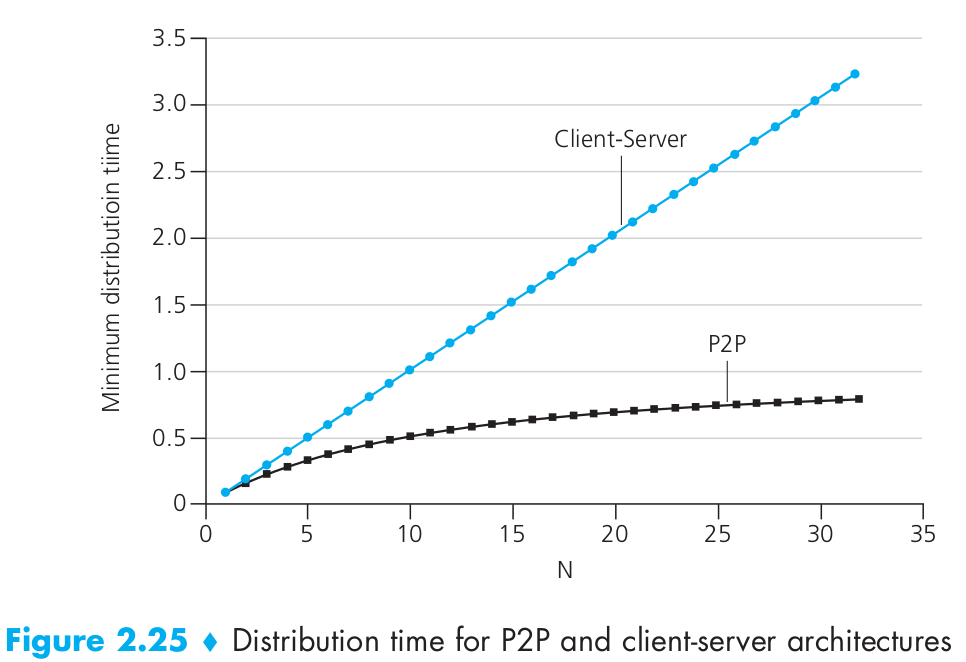
\includegraphics[width=89mm]{imagenes/Escalabilidad}
\end{figure}

\section{BitTorrent} 

BitTorrent es un protocolo P2P para distribución de archivos. El
conjunto de peers que participan en la comunicación se llama
\textit{torrent}. Los peers en un torrent descargan chunks de igual
tamaño del archivo (típicamente 256 Kbytes). Al principio, un
peer no tiene ningún chunk y va acumulándolos con el paso del tiempo a la vez que va difundiendo los que ya tiene al resto de peers. Un peer puede, en cualquier momento, abandonar el torrent con un subconjunto de chunks del archivo y volver a conectarse en otro momento para reanudar la comunicación. Una vez descargado el archivo, un peer puede seguir en el torrent compartiéndolo o abandonar la red.\\

\begin{figure}[H]
  \centering
  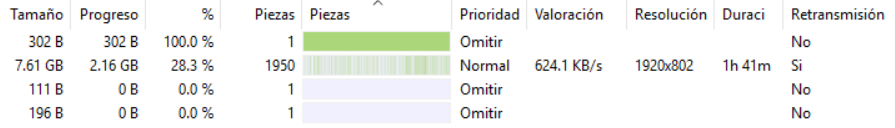
\includegraphics[width=139mm]{imagenes/piezasUtorrent}
  \caption{ Captura de $\mu$Torrent: Se observa un archivo con 1950 chunk, de los cuales sólo se han descargado algunos.}
\end{figure}

El principal mecanismo de BitTorrent es el siguiente:

Un archivo con la extensión \texttt{.torrent}, que contiene
información sobre el archivo a descargar (nombre, logitud, información
de hashing) y la url de un \textit{tracker} (un servidor que asiste a
la comunicación entre peers en el torrent), se sube a un servidor
web. Un usuario ejecuta el \texttt{.torrent} en un cliente para unirse
al torrent. Cuando un peer se une, a través de un protocolo basado en
HTTP, manda información al tracker sobre qué archivo está descargando
y cuál es su puerto de escucha, entre otras cosas. Periódicamente los
peers le informan de que siguen activos para que el tracker lleve un registro de los peers participantes. Cuando se une un peer, el tracker le envía la IP de un subconjunto de peers elegido aleatoriamente, con los que intenta establecer comunicación TCP. Los peers con los que establece comunicación TCP (``vecinos'') pueden dejar el torrent, y también pueden conectarse con él nuevos peers. Periódicamente, cada peer solicita a sus vecinos la lista de chunks que tienen (por conexión TCP) y luego solicita chunks que no tiene.\\

Para determinar que chunk solicitar primero se usa la \textbf{heurística del más raro}. De entre los chunks que no tiene, el peer solicita aquel que menos se repita entre las listas de chunks de sus vecinos, con el fin de equilibrar el número de copias de cada chunk en el torrent. De esta forma se reduce el riesgo de que todos los peers que tienen un chunk estén desconectados simultáneamente.\\

Para decidir que solicitudes atender, un peer da prioridad a los vecinos que actualmente le proporcionan más datos. Cada peer determina los cuatro peers que más datos le comparten, basándose en la media de los últimos 20 segundos, y es a éstos a los que atiende (se les llama \textit{unchoked peers}). Este top cuatro se recalcula cada 10 segundos. Además, cada peer escoge adicionalmente uno de sus vecinos al azar y atiende sus peticiones (\textbf{Optimistic Unchoking}). Éste vecino se recalcula cada 30 segundos. De esta forma, los nuevos peers en el torrent consiguen chunks para intercambiar, y así ascender a los cuatro vecinos favoritos de algunos peers y permite encontrar mejores conexiones. A largo plazo, este criterio provoca que los peers que comparten información a velocidades similares se encuentren mutuamente.\\

Este sistema presenta una gran escalabilidad ya que su cuello de
botella es la sobrecarga del ancho de banda del tracker, pero la
función de éste requiere muy poco ancho de banda.

\subsection{Otros mecanismos de funcionamiento:}

\begin{itemize}
\item \textbf{Pipelining y mini-chunks:} En una conexión TCP, es
  importante tener siempre varias solicitudes pendientes para evitar
  el retraso entre chunks enviados. BitTorrent facilita ésto
  subdiviendo los chunks en piezas más pequeñas (normalmente 16
  Kbytes) y manteniendo algunas solicitudes (normalmente cinco) en un
  pipeline. Cada vez que una sub-pieza (mini-chunk) llega a su
  destinatario, éste manda una nueva solicitud.

\item Se da \textbf{Prioridad Estricta} a los mini-chunks que forman
  parte de un chunk del que ya se han descargado algunos
  mini-chunks. Esto ayuda a que se consigan chunks completos lo más
  rápido posible.
  
\item \textbf{Primera Pieza Aleatoria:} Cuando un peer se une al
  torrent por primera vez, no tiene nada que compartir. Su prioridad
  debe ser conseguir un chunk completo lo antes posible. Si solicitase
  el chunk más raro, tendría pocas fuentes de las cuales descargar
  mini-chunks y la descarga sería más lenta. Es por eso que las piezas
  a descargar se solicitan aleatoriamente hasta que se consiga el
  primer chunk completo. Una vez conseguido, se cambia a la heurística
  del más raro.
  
\item \textbf{Endgame Mode:} Cuando un peer tiene solicitadas todas
  las sub-piezas que le faltan, solo le queda esperar a que se las
  envíen. Si una de ellas se envía a baja velocidad, el peer
  desperdicia ancho de banda. Para evitar esto, el peer solicita todas
  las mini-piezas restantes a todos los peers y va cancelando
  solicitudes conforme las vaya recibiendo. De esta manera, a cambio
  de un desperdicio del ancho de banda por un corto periodo de tiempo,
  el archivo se termina de descargar rápidamente.
  
\item \textbf{Anti-Snubbing:} Cuando un peer deja de recibir chunks de
  sus vecinos, empieza a tener una velocidad de descarga baja hasta
  que encuentre nuevos peers adecuados, cosa que sólo puede hacer por
  medio de Optimistic Unchoking. BitTorrent considera que un peer que
  lleva más de un minuto sin descargar un chunk desde un peer
  particular está siendo despreciando (\textit{``snubbed''}) por éste
  y deja de enviarle piezas a no ser que lo encuentre con Optimistic
  Unchoking. Esto frecuentemente resulta en más de un Optimistic
  Unchoke simultáneo (una excepción). De esta manera se recuperan más
  rápido los ratios de descarga.

\item \textbf{Sólo subida:} Una vez que un peer ha descargado el
  archivo completo, ya no hace uso de su velocidad de bajada. Entonces
  pasa a enviar chunks a los peers que mejor aprovechan su capacidad
  de subida, priorizando aquellos a los que nadie más les está
  compartiendo.

\item \textbf{UDP Tracker:} Una extensión reciente de BitTorrent es el
  UDP Tracker Protocol. El tracker usa el protocolo UDP para la
  transmisión de datos, en vez del protocolo HTTP (sobre TCP). Esto
  tiene mejor rendimiento y menor sobrecarga en el tracker, pero no
  todos los clientes de BitTorrent lo soportan. Aun así, usa TCP como
  protocolo de transporte.
  
\end{itemize}

\section{Capturas con Wireshark}

En esta sección usaremos la herramienta Wireshark para ver el intercambio de paquetes al utilizar BitTorrent. Descargamos un torrent con el cliente Transmission. BitTorrent es un protocolo que no está encriptado por defecto, pero la mayoría de clientes permite encriptar el tráfico. Veremos que en nuestro caso lo encripta.

\subsection{Conexión con Tracker}

Nos centraremos en la conexión con los trackers.

\begin{figure}[H]
  \centering
  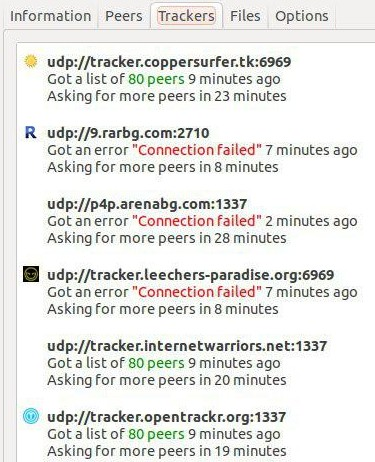
\includegraphics[width=64mm]{imagenes/tracker_transmission}
  \caption{Captura de Transmision: Lista de los trackers a los que nos conectamos para descargar el archivo.}
\end{figure}

\begin{figure}[H]
  \centering
  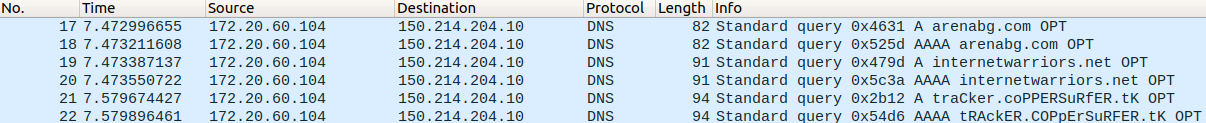
\includegraphics[width=150mm]{imagenes/trackers}
  \caption{Captura de Wireshark: Conexión con trackers.}
\end{figure}

\begin{figure}[H]
  \centering
  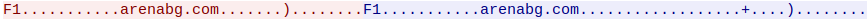
\includegraphics[width=150mm]{imagenes/arenabg}
  \caption{Captura de Wireshark: Intercambio de mensajes para la conexión al tracker ``arenabg''. Estos mensajes se hacen con protocolo DNS, que usa UDP internamente.}
\end{figure}

\begin{figure}[H]
  \centering
  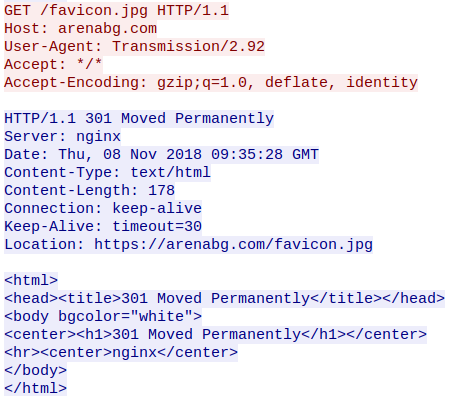
\includegraphics[width=54mm]{imagenes/tcp-http-arenabg}
  \caption{Captura de Wireshark: Usando el protocolo HTTP, nos comunicamos con el tracker.}
\end{figure}

\begin{figure}[H]
  \centering
  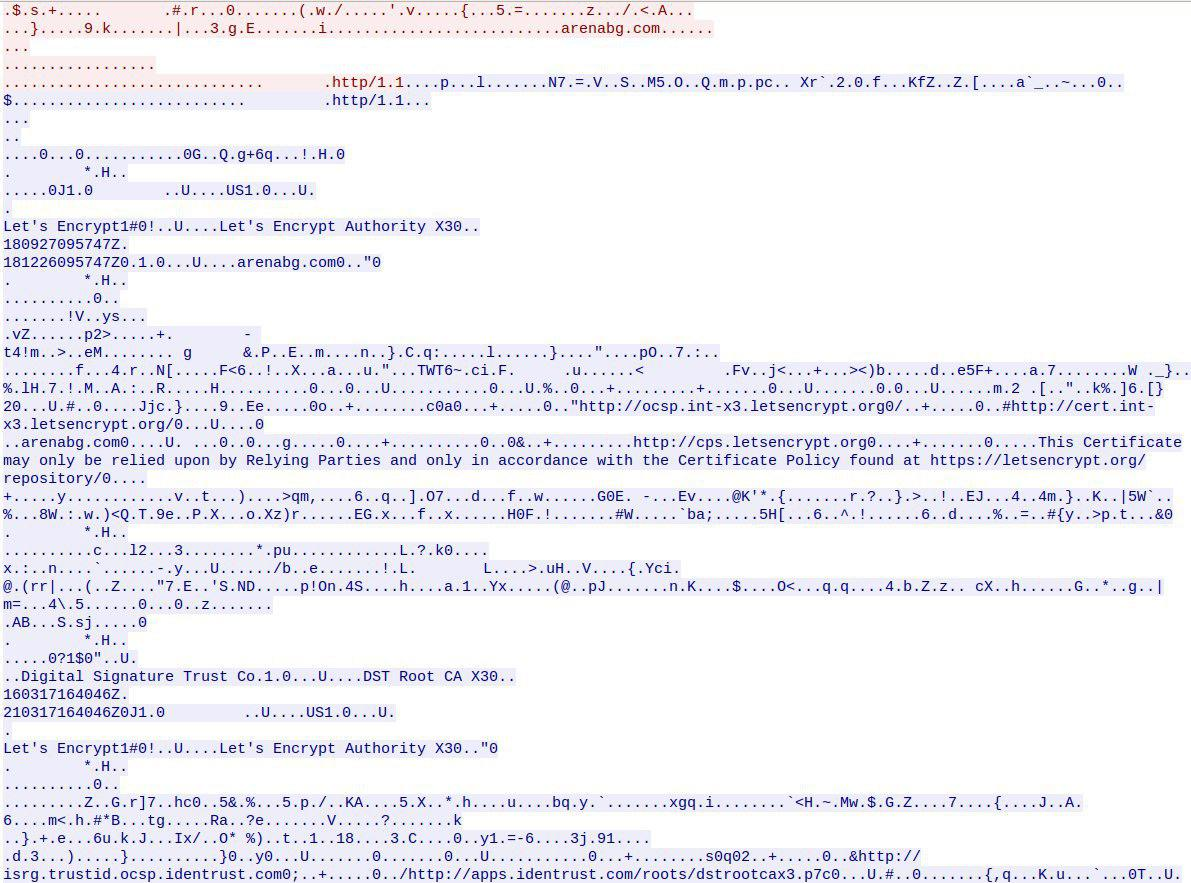
\includegraphics[width=127mm]{imagenes/trama_arenabg}
  \caption{Captura de Wireshark: Vemos como, tras el saludo, el tracker nos envía ``Let's Encrypt'', para empezar a encriptar los mensajes y \texttt{``..arenabg.com0....U. ...0..0...g.....0....+..........0..0\&..+.........http://cps.letsencrypt.org0....+.......0.....This Certificate may only be relied upon by Relying Parties and only in accordance with the Certificate Policy found at https://letsencrypt.org/repository/0....''}, donde le manda el nombre del tracker (arenabg) y su política. Esto se hace con TCP. Tras esto empieza la conversación.}
\end{figure}

\subsection{Conexión con Peers}
En las siguientes imágenes mostraremos la conexión con los peers y el intercambio de chunks con estos.

\begin{figure}[H]
  \centering
  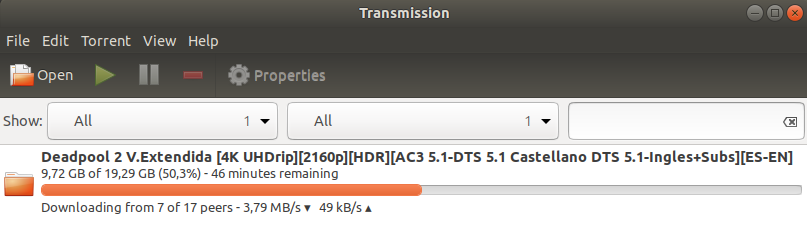
\includegraphics[width=139mm]{imagenes/transmission-deadpool}
  \caption{Captura de Transmision: Descargamos paquetes de 7 de los 17 peers disponibles. La velocidad de subida es 49 KBytes/s y la de bajada 3,79 MBytes/s.}
\end{figure}


\begin{figure}[H]
  \centering
  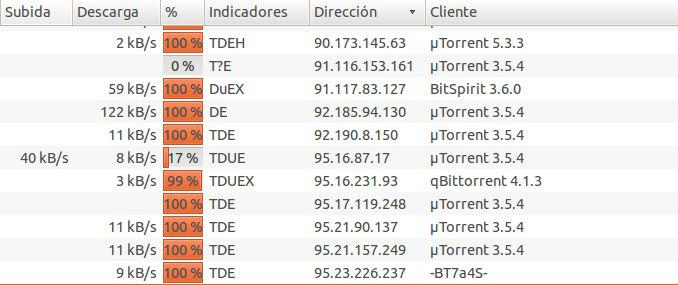
\includegraphics[width=139mm]{imagenes/peers}
  \caption{Captura de Transmision: Los peer con los que nos estamos comunicando, nuestros ``vecinos''. Por ejemplo, del peer 92.185.94.130 estamos descargando paquetes a una velocidad de 122 KBytes/s. Además estamos enviando chunks al peer 95.16.87.17 a 40 KBytes/s.}
\end{figure}

\begin{figure}[H]
  \centering
  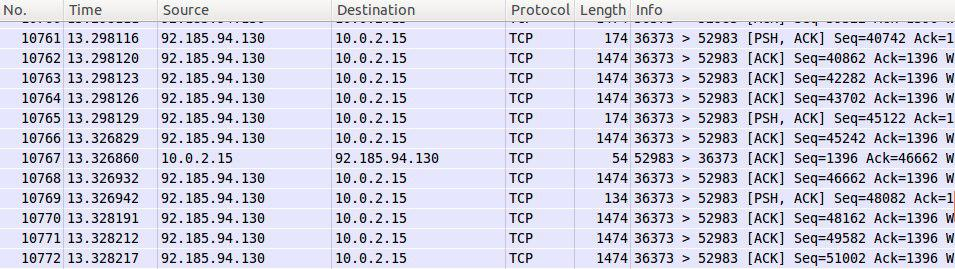
\includegraphics[width=139mm]{imagenes/TCP_wireshark}
  \caption{Captura Wireshark: El peer del ejemplo anterior (el 92.185.94.130) nos está pasando paquetes TCP con muchos datos y nosotros le respondemos con paquetes de menor longitud.}
\end{figure}

A continuación vemos un trozo de una conversación de tamaño 1413129 bytes. Al principio hay un intercambio de información entre ambos peers y luego la fuente empieza a enviar chunks.
Hay que tener en cuenta que el archivo que estamos descargando es un archivo de vídeo y el intercambio de mensajes está encriptado.

\begin{figure}[H]
  \centering
  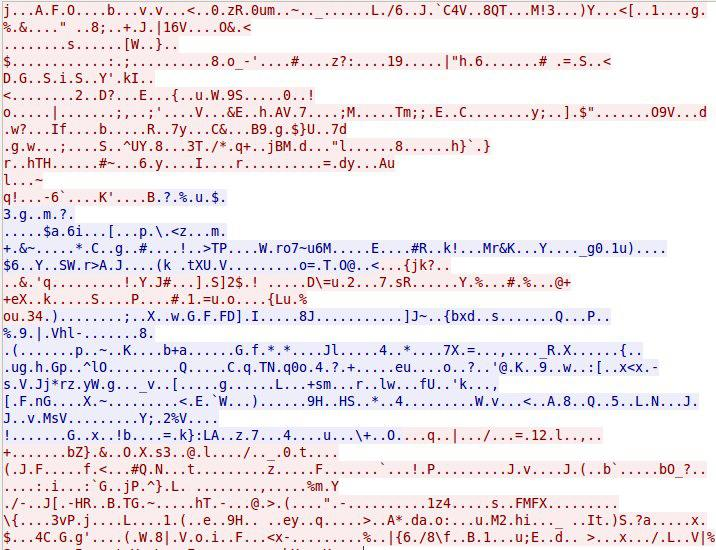
\includegraphics[width=84mm]{imagenes/trama_rojo}
  \caption{Vemos el intercambio de información entre los peers. Lo que envía la fuente aparece en azul y lo que envía nuestro host en rojo.}
\end{figure}

\begin{figure}[H]
  \centering
  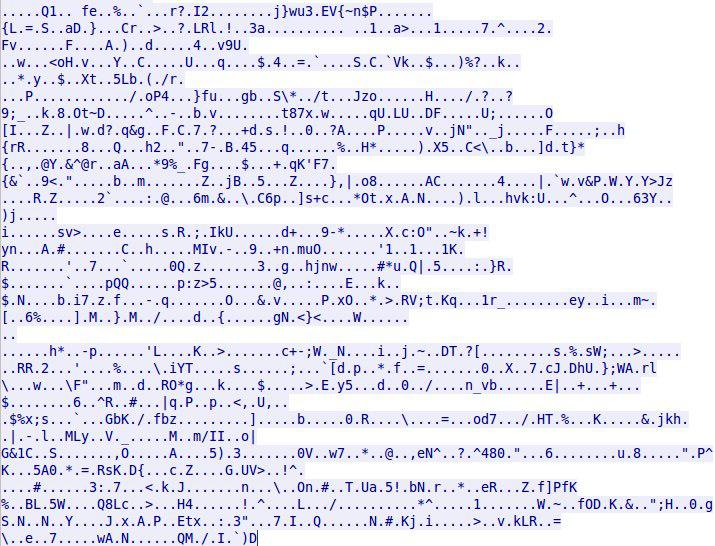
\includegraphics[width=84mm]{imagenes/trama_azul}
  \caption{El resto de la conversación aparece en azul hasta completar los 1413129 bytes.}
\end{figure}

Para obtener un análisis secuencial de las conexiones TCP, consultamos el gráfico de flujo TCP:

\begin{figure}[H]
  \centering
  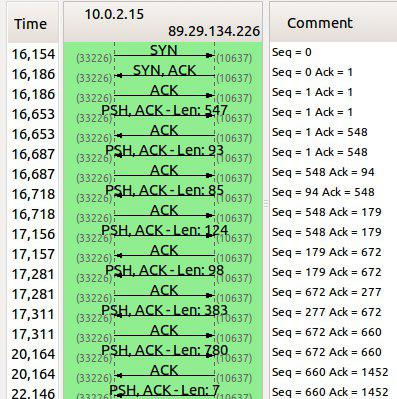
\includegraphics[width=59mm]{imagenes/statistic_flow}
  \caption{Nótese que las tres primeras líneas muestran el establecimiento de la conexión: ``SYN'', ``SYN ACK'', ``ACK'', lo que es llamado 3-Way Handshake}
\end{figure}

\begin{figure}[H]
  \centering
  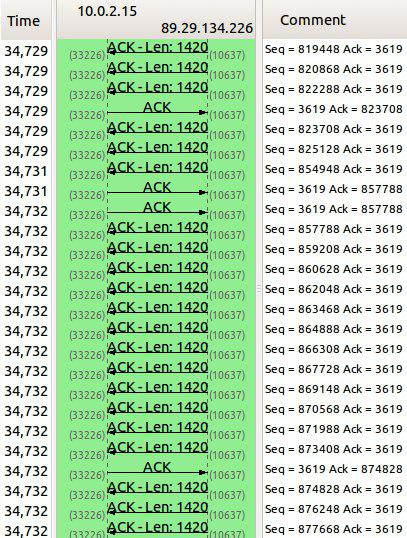
\includegraphics[width=59mm]{imagenes/statistic_flow1}
  \caption{La fuente envía chunks al host y el host confirma que los recibe}
\end{figure}

\section{Referencias}
\begin{itemize}
\item \href{https://en.wikipedia.org/wiki/BitTorrent}{https://en.wikipedia.org/wiki/BitTorrent}
\item Jim Kurose, Keith Ross, \href{https://www.bau.edu.jo/UserPortal/UserProfile/PostsAttach/10617_1870_1.pdf}{``Computer Networking: A Top-Down Approach''}, Pearson, 2013, pp. 144-151.
\item Bram Cohen, \href{http://bittorrent.org/bittorrentecon.pdf}{``Incentives Build Robustness in BitTorrent''}, 2003.
\item \href{https://wiki.wireshark.org/BitTorrent}{https://wiki.wireshark.org/BitTorrent}
\item \href{https://en.wikipedia.org/wiki/UDP_tracker}{https://en.wikipedia.org/wiki/UDP\_tracker}
\end{itemize}    

\end{document}